\section{PO-Gitlab and CI tools}
\label{sec:PO-Gitlab_and_CI_tools}

The Physics Office GitLab project aims to simplify the ATLAS documents (Papers, CONF notes, PUB notes and internal notes) creation, editing and publication process by using the tools provided by the CERN GitLab system. The usual publication workflow consisted on a heavy e-mail communication between ATLAS editors and Physics Office in order to ensure that ATLAS rules were being followed before being able to submit the desired paper to arXiv or to the journal of choice. This approach lead, usually, to modifications done in different sides (Officers and editors) not properly implemented by the other side that slows down the process due to small details, which with a different approach would be easily fixed. 
There are three main areas modified by the PO-GitLab approach with the goal of simplifying this process. These areas are the automatic creation of the document GitLab projects (git repositories in a centralised way), the real-time verification by the GitLab Continuous Integration (CI) tools of the documents being written and the automatic processing of the document to ensure an accurate publication process. These areas are described in this section. 

\subsection{Automatic document creation}
\label{sec:Automatic_document_creation}

First, a centralised area controlled by ATLAS Physics Office needs to be designed. The control is key in order to allow Physics Office to maintain quality controls over the document being accepted for publication.

A basic structure is already set in Gitlab to store the groups related to an Analysis. The main Gitlab group is called atlas-physics-office and it stores many subgroups. Each of those subgroups belong to a leading group, for example: Higgs, Exotics, SUSY etc., see Fig.~\ref{fig:Gitlab_repository}.

Having this structure defined, it is possible to automatically create documents through Fence thanks to the communication between the framework and the Gitlab API in the so called FENCE and Gitlab integration, better explained in section~\ref{sec:FENCE_and_Gitlab_integration}. This amortisation relies on file templates that has its variables substituted according to the related publication. This way, all the created repositories contain the default documents correctly formatted to start writing a Paper, CONF, PUB or an internal note. The repository is also configured with all the needed branches, labels and also placed in the correct Gitlab group.

\subsection{Real-time check with GitLab’s CI}
\label{sec:Real-time_check_with GitLabs_CI}

GitLab CI tools are designed to execute a set of automatic tasks every time a new modification is introduced in the document (i.e. a new commit is pushed to the document repository). The approach from Physics Office was to develop a package that is able to run different jobs on a given document by verifying distinct aspects, which is performed by the pogitlab python package~\cite{pogitlab-repo}. Given the modularity of the system, new and/or more complex tasks can me added, ensuring scalability.    
                    
GitLab’s CI works through Pipelines. Each time a new commit is pushed to the repository, a pipeline is triggered. A pipeline is a set of jobs grouped in stages. All the jobs in the same stage are executed in parallel while each stage is only executed once the previous one has finished. The real-time verifications are performed in most of the branches of the project and they are called edit-pipelines.
\begin{figure}[ht!]
  \centering
  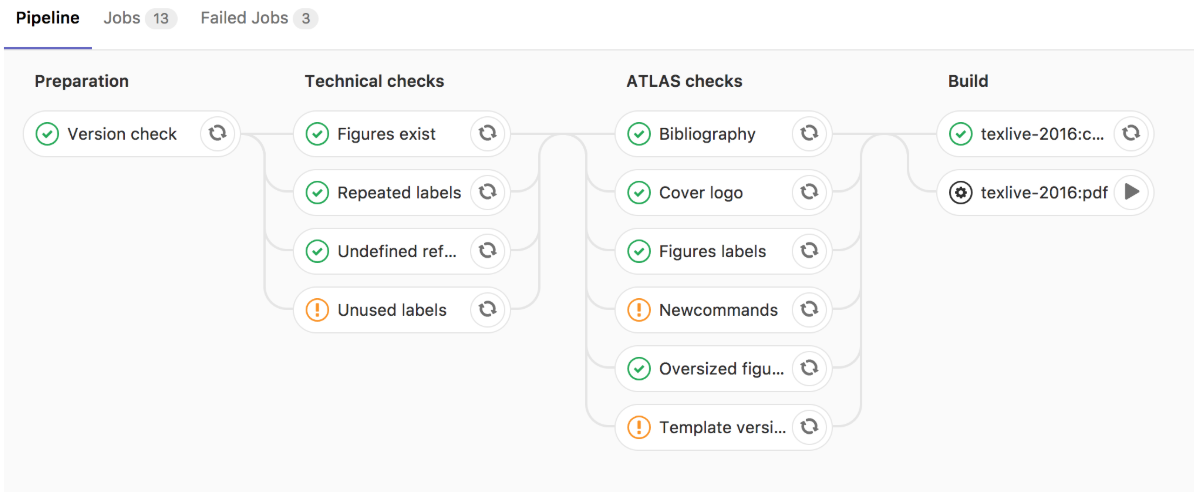
\includegraphics[width=0.9\textwidth]{figures/editing_pipelines_1.png}
  \caption{Screenshot of editing pipelines.}
  \label{fig:editing_pipelines_1}
\end{figure}

Fig.~\ref{fig:editing_pipelines_1}, presents an example of the edit-pipelines that consist in the following set of stages:
\begin{itemize}

\item \textbf{Preparation}: It consist of only one job that checks the current version of the PO-Gitlab package. 

\item \textbf{Technical checks}: This stage includes checks related to LATEX:

    {\begin{itemize}
    \item Figures exist: check if all figures used throughout the document are present in the repository or if anyone is missing.
    \item Files exist: check if all the .tex files included in the document are present.
    \item Repeated commands: checks for repeated user defined commands. It is not wise to use the same command for different purposes and can be an issue when generating captions for figures and tables for the ATLAS public pages.
    \item Repeated labels: checks for duplicate labels all documents.
    \item Undefined references: checks for undefined references.
    \item Unused labels: warnings against label which has been defined but not used. Although this is not an issue it might point to something not being properly referenced.
    \end{itemize}}
    
\item \textbf{ATLAS checks}: These are checks related to ATLAS rules and style:

    {\begin{itemize}
    \item Bibliography: checks that the bibliography files are included.
    \item Cover logo: checks that the proper logo is being used in the ATLAS template.
    \item Figures labels: checks for labels in figures depending on the type of document. Table~\ref{tab1} shows the different labels which are allowed and not allowed in different files.
    \item Oversized figures: checks for figures larger than 2 Mb.
    \item Preprint ID: checks that the preprint ID is included in the document.
    \item Template version: checks that the version of the ATLAS LATEX template is the latest one available.
    \item Title and Abstract: checks that no user-defined commands (i.e. not LATEX commands) are being used nor in the title neither in the abstract.
   \end{itemize}}
   
\item \textbf{Build}: this stage builds the document itself. The pdf of the document is not usually saved to avoid increase in size of the repository but a manual job (only run when manually asked) builds the document and saves the pdf as an artifact for the user to download.
\end{itemize}
\begin{table}[ht!]
\centering
\begin{tabular}{|c|c|c|}\hline
   Document type & Preliminary label & Internal label \\
  \hline\hline
   PAPER & Not allowed & Not allowed \\
  \hline
    BOOK & Not allowed & Not allowed \\
  \hline
    CONF & Allowed & Not allowed \\
  \hline
    PUB & Allowed & Not allowed \\
  \hline
    NOTE & Allowed & Allowed \\
  \hline \hline
\end{tabular}
\caption{\label{tab1}Labels allowed and not allowed in figures depending on the document type.
1 The files and figures exist checks are needed because it is rather common to forget committing a new file or figure.}
\end{table}

The GitLab’s CI also produces the required files for the paper submission, using dedicated pipelines, similar to the editing ones. In this case, a protected git branch, named PO-ready, is created by default at the time of the setup of the paper repository. Any PO-* branch will trigger the paper submission pipelines. Such pipelines have the previously described tests, but after at the build stage a flattening of the LaTeX document happens, allowing the following actions:

\begin{enumerate}
\item all the source files are merged into a single LaTeX source file;
\item all the comments in the LaTeX source file are removed;
\item all the figures are renamed following the convention required by the APS journals;
\item any directory structure is removed;
\end{enumerate}
As shown in Fig.~\ref{fig:editing_pipelines_2}.

Furthermore, tarballs suitable for submission to arXiv and APS journals are created using TeXlive 2016 and 2017, respectively, and a tarball with the required files for the public webpage with plots and tables is created. These tarballs are created as gitlab artifacts and can be downloaded by the members of the Physics Office and editors. In the submission tarballs, the auxiliary material (figures and tables not for submission) are not included.
\begin{figure}[ht!]
  \centering
  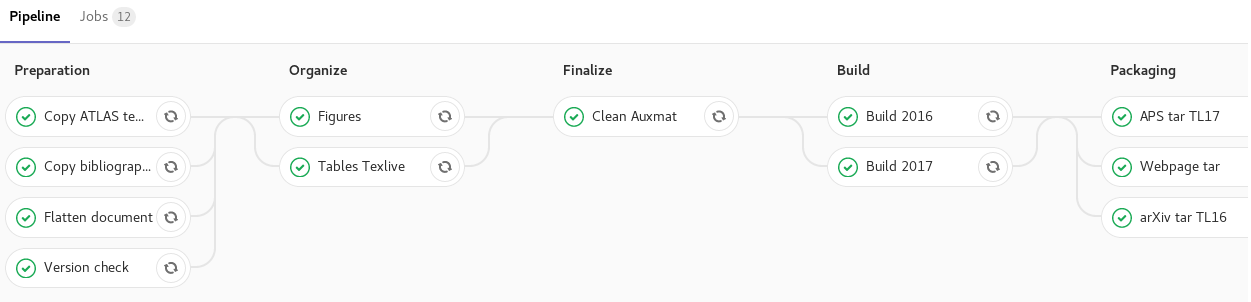
\includegraphics[width=0.9\textwidth]{figures/editing_pipelines_2.png}
  \caption{Screenshot of editing pipelines.}
  \label{fig:editing_pipelines_2}
\end{figure}


